\begin{center}
	\section{Sedimentaci\'on}
\end{center}

\noindent
\justify

La sedimentaci\'on es uno de los procesos m\'as antiguos en el tratamiento del agua y consiste en la deposici\'on de materiales s\'olidos de mayor peso que el agua.

\noindent
\justify

Existen cinco tipos de sedimentaci\'on que se clasifican de acuerdo a  la clase de part\'icuas, caracter\'isticas superficiales y concentraci\'on de las mismas:

\begin{itemize}
	\item Sedimentaci\'on \textit{discreta:} las part\'iculas no tienden a aglomerarse, mantienen su tama\~no e individualidad. Son generalmente de textura arenosa.
	\item Sedimen \textit{floculenta}: las part\'iculas floculan y tienden a agruparse durante el proceso.
	\item Sedimentaci\'on \textit{m\'asica}: la concentraci\'on de part\'iculas es tan grande que colisionan entre s\'i, sedimentando como una masa.
	\item Sedimentaci\'on por \textit{compresi\'on}: la concentraci\'on de part\'iculas es tan grande que cada una reposa sobre la otra, present\'andose una especie de soporte entre cada una de ellas; el peso de las part\'iculas superiores tiende a compactar a las inferiores.
	\item Sedimentaci\'on de \textit{alta tasa}: es una variaci\'on de la sedimentaci\'on discreta, en la que se insertan placas paralelas con el fin de aumentar la eficiencia de remoci\'on de part\'iculas.
\end{itemize}

\noindent
\justify

La \textit{sedimentaci\'on} realiza la separaci\'on de los s\'olidos m\'as densos que el agua y la \textit{filtraci\'on} separa aquellos que tienen una densidad muy cercana a la del fluido.

\subsection{Sedimentaci\'on con coagulantes}

\noindent
\justify

Se efect\'ua la decantaci\'on de part\'iculas en las c\'amaras de floculaci\'on; el tama\~no y densidad de las part\'iculas y viscosidad del agua desempae\~nar\'an un papel importante en el dimensionamiento de los sedimentadores. Las unidades podr\'an ser circulares o de flujo radial, cuadradas y rectangulares. Si los tanques sedimentadores se dise\~nan en dos o m\'as pisos, podr\'an ser de flujos independientes o de flujo \textit{zig-zag}, de manera que el flujo recorra todos los pisos de la unidad.

\subsection{Sedimentadores de \textit{placas paralelas}}

\noindent
\justify

Se trata de un tipo de sedimentador desarrollado por Hazen A, en 1904, quien expuso el siguiente principio: ``como la acci\'on de un tanque sedimentador depende de su \'area, y no de su profundidad, una subdivisi\'on horizontal producir\'ia una superficie doble para reunir sedimentos en lugar de una sencilla y duplicar\'ia la cantidad de trabajo". 

\noindent
\justify

La diferencia de los sedimentadores de tasa normal y los de alta tasa son:

\begin{itemize}
	\item El fondo del decantador no es horizontal sino inclinado.
	\item La profundidad del decantador es baja, de forma que hay que construir un n\'umero considerable de celdas superpuestas para poder tratar los vol\'umenes de agua.
	\item El flujo \textbf{debe ser laminar}, con n\'umero de Reynolds entre $80$ y $250$.
\end{itemize}

\begin{figure}[h!]
	\centering
	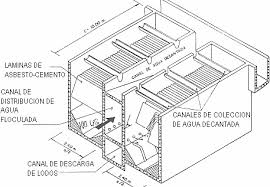
\includegraphics[width=0.7\textwidth]{Images/Sedimentacion/placas.jpg}
	\caption{Sedimentador de placas paralelas.}
	\label{placas}
\end{figure}

\noindent
\justify

Las placas presentan una inclinaci\'on, donde el agua ascendente deposita sobre ellas el material que trae en suspensi\'on. Los lodos resbalan pendiente abajo, y pueden ser recolectados en una tolva en la parte inferior de la estructura.

\begin{equation}
	V_s = \frac{V_0 S}{\sin \theta + \frac{L}{e} \cos \theta}
	\label{CargaSuperficial}
\end{equation}

\noindent
\justify

La Ecuaci\'on \ref{CargaSuperficial}, para un determinado posicionamiento de las placas, permite determinar la velocidad requerida para conseguir una velocidad cr\'itica. Es crucial mantener el n\'umero de Reynolds bajo para evitar que la turbulencia levante los lodos de la cara de las placas donde se est\'a sedimentando.

\subsection{Turbiedad}

\noindent
\justify

La turbidez es la expresi\'on de la propiedad \'optica de la muestra que causa que los rayos de la luz sean dispersados y absorbidos en lugar de ser transmitidos en l\'inea recta a trav\'es de la muestra.

\noindent
\justify

La turbiedad en el agua puede ser causada por la presencia de part\'iculas suspendidas y disueltas de gases, l\'iquidos y s\'olidos tanto org\'anicos como inorg\'anicos.

\noindent
\justify

La eliminaci\'on de la turbiedad se lleva a cabo mediante procesos de coagulaci\'on, asentamiento y filtraci\'on.
